
\subsection{First Day TOPP Value Comparison} \label{ss:day1} %first day comparison

\begin{figure}
    \centering
    \includegraphics[width=\textwidth]{img/first_day_values}
    \vspace{0mm}
    \caption{First day TOPP values obtained using (a) MCM v3.1, (b) CRI v2, \mbox{(c) MOZART-4}, (d) RADM2, (e) RACM, (f) RACM2, (g) CBM-IV and (h) CB05 mechanisms compared to the corresponding MCM v3.2 values.}
    \vspace{-4mm}
    \label{f:first_day}
\end{figure}

\begin{figure}
    \centering
    \includegraphics[width=\textwidth]{img/Ox_tagged_budget_overlay_all_mechanisms}
    \vspace{0mm}
    \caption{\ce{O_x} production budgets allocated to individual VOCs using (a) MCM v3.2, \mbox{(b) MCM v3.1}, (c) CRI v2, (d) RADM2, (e) RACM, (f) RACM2, (g) MOZART-4, \mbox{(h) CBM-IV} and (i) CB05 mechanisms.}
    \vspace{-4mm}
    \label{f:Ox_tagged_budgets}
\end{figure}

The first day TOPP values calculated from each mechanism are compared to those calculated with the MCM v3.{2} in Figure \ref{f:first_day}. 
The reduced mechanisms generally match the MCM v3.2 first day TOPP values. 
However the TOPP values resulting from aromatic VOC degradation are lower in reduced mechanisms.

Aromatic chemistry is difficult to represent in chemical mechanisms as many products, their yields and reactions are not known or are subject to uncertainties \citep{Vereecken:2012}. 
Thus, greater variation is expected between the aromatic VOC TOPP values.
The largest discrepancies are the zero TOPP values of toluene and xylene in RACM. 
This is unrealistic as aromatic VOCs contribute significantly to \ce{O_x} production \citep{Derwent:1998}. 
Section \ref{sss:aromatic} outlines the responsible chemistry.

The $2$-methylpropene first day TOPP values in RACM, RACM2, CBM-IV and CB05 indicate that its degradation is treated very differently to the MCM v3.2. 
The variation between RACM, RACM2 and MCM v3.2 arise from differences between the rate constants of $2$-methylpropene ozonolysis. 
These rate constants are derived from the IUPAC recommendations \citep{IUPAC_Site}, however RACM and RACM2 rate constants are an order of magnitude faster than the MCM v3.2.
This results from the rate constant being a weighted mean of all VOC ozonolysis rate constants represented as OLI in RACM and RACM2 \citep{Stockwell:1997, Goliff:2013}.
The resulting increased radical production leads to more \ce{O_x} production than in the MCM v3.2.

In CBM-IV, $2$-methylpropene is represented by the mechanism species ALD2 \citep{Hogo:1989}, which is a surrogate for aldehydes with more than one carbon atom. 
ALD2 reacts very quickly with OH forming \ce{CH3CO3}, leading to \ce{O_x} production. 
Furthermore, photolysis of ALD2 promotes radical and in turn \ce{O_x} production. 
This is not a degradation pathway for $2$-methylpropene in any other mechanism. 
The choice of $2$-methylpropene representation gives rise to higher \ce{O_x} production than in the MCM v3.2.

$2$-methylpropene representation was updated in CB05 to \mbox{FORM + $3$ PAR}, where FORM represents formaldehyde and PAR the paraffin \ce{C-C} bond \citep{Yarwood:2005}. 
The initial oxidation reactions of formaldehyde are similar to ALD2 whilst PAR is a slow reacting species. 
This slows down the \ce{O_x} production resulting in lower \ce{O_x} production than in the MCM v3.2.

The first day TOPP values of many VOCs using CBM-IV and CB05 are lower than those of the MCM v3.2. 
This is related to lower \ce{O_x} production in CBM-IV and CB05, shown in Figure \ref{f:Ox_tagged_budgets}.
Lower \ce{O3} levels using CBM-IV and CB05 have also been noted in other modelling studies such as \citet{Luecken:2008, Emmerson:2009} and \citet{Saylor:2012}.

\subsection{TOPP Value Time Series} \label{ss:profiles} %TOPP time series of all species

\begin{figure}
    \centering
    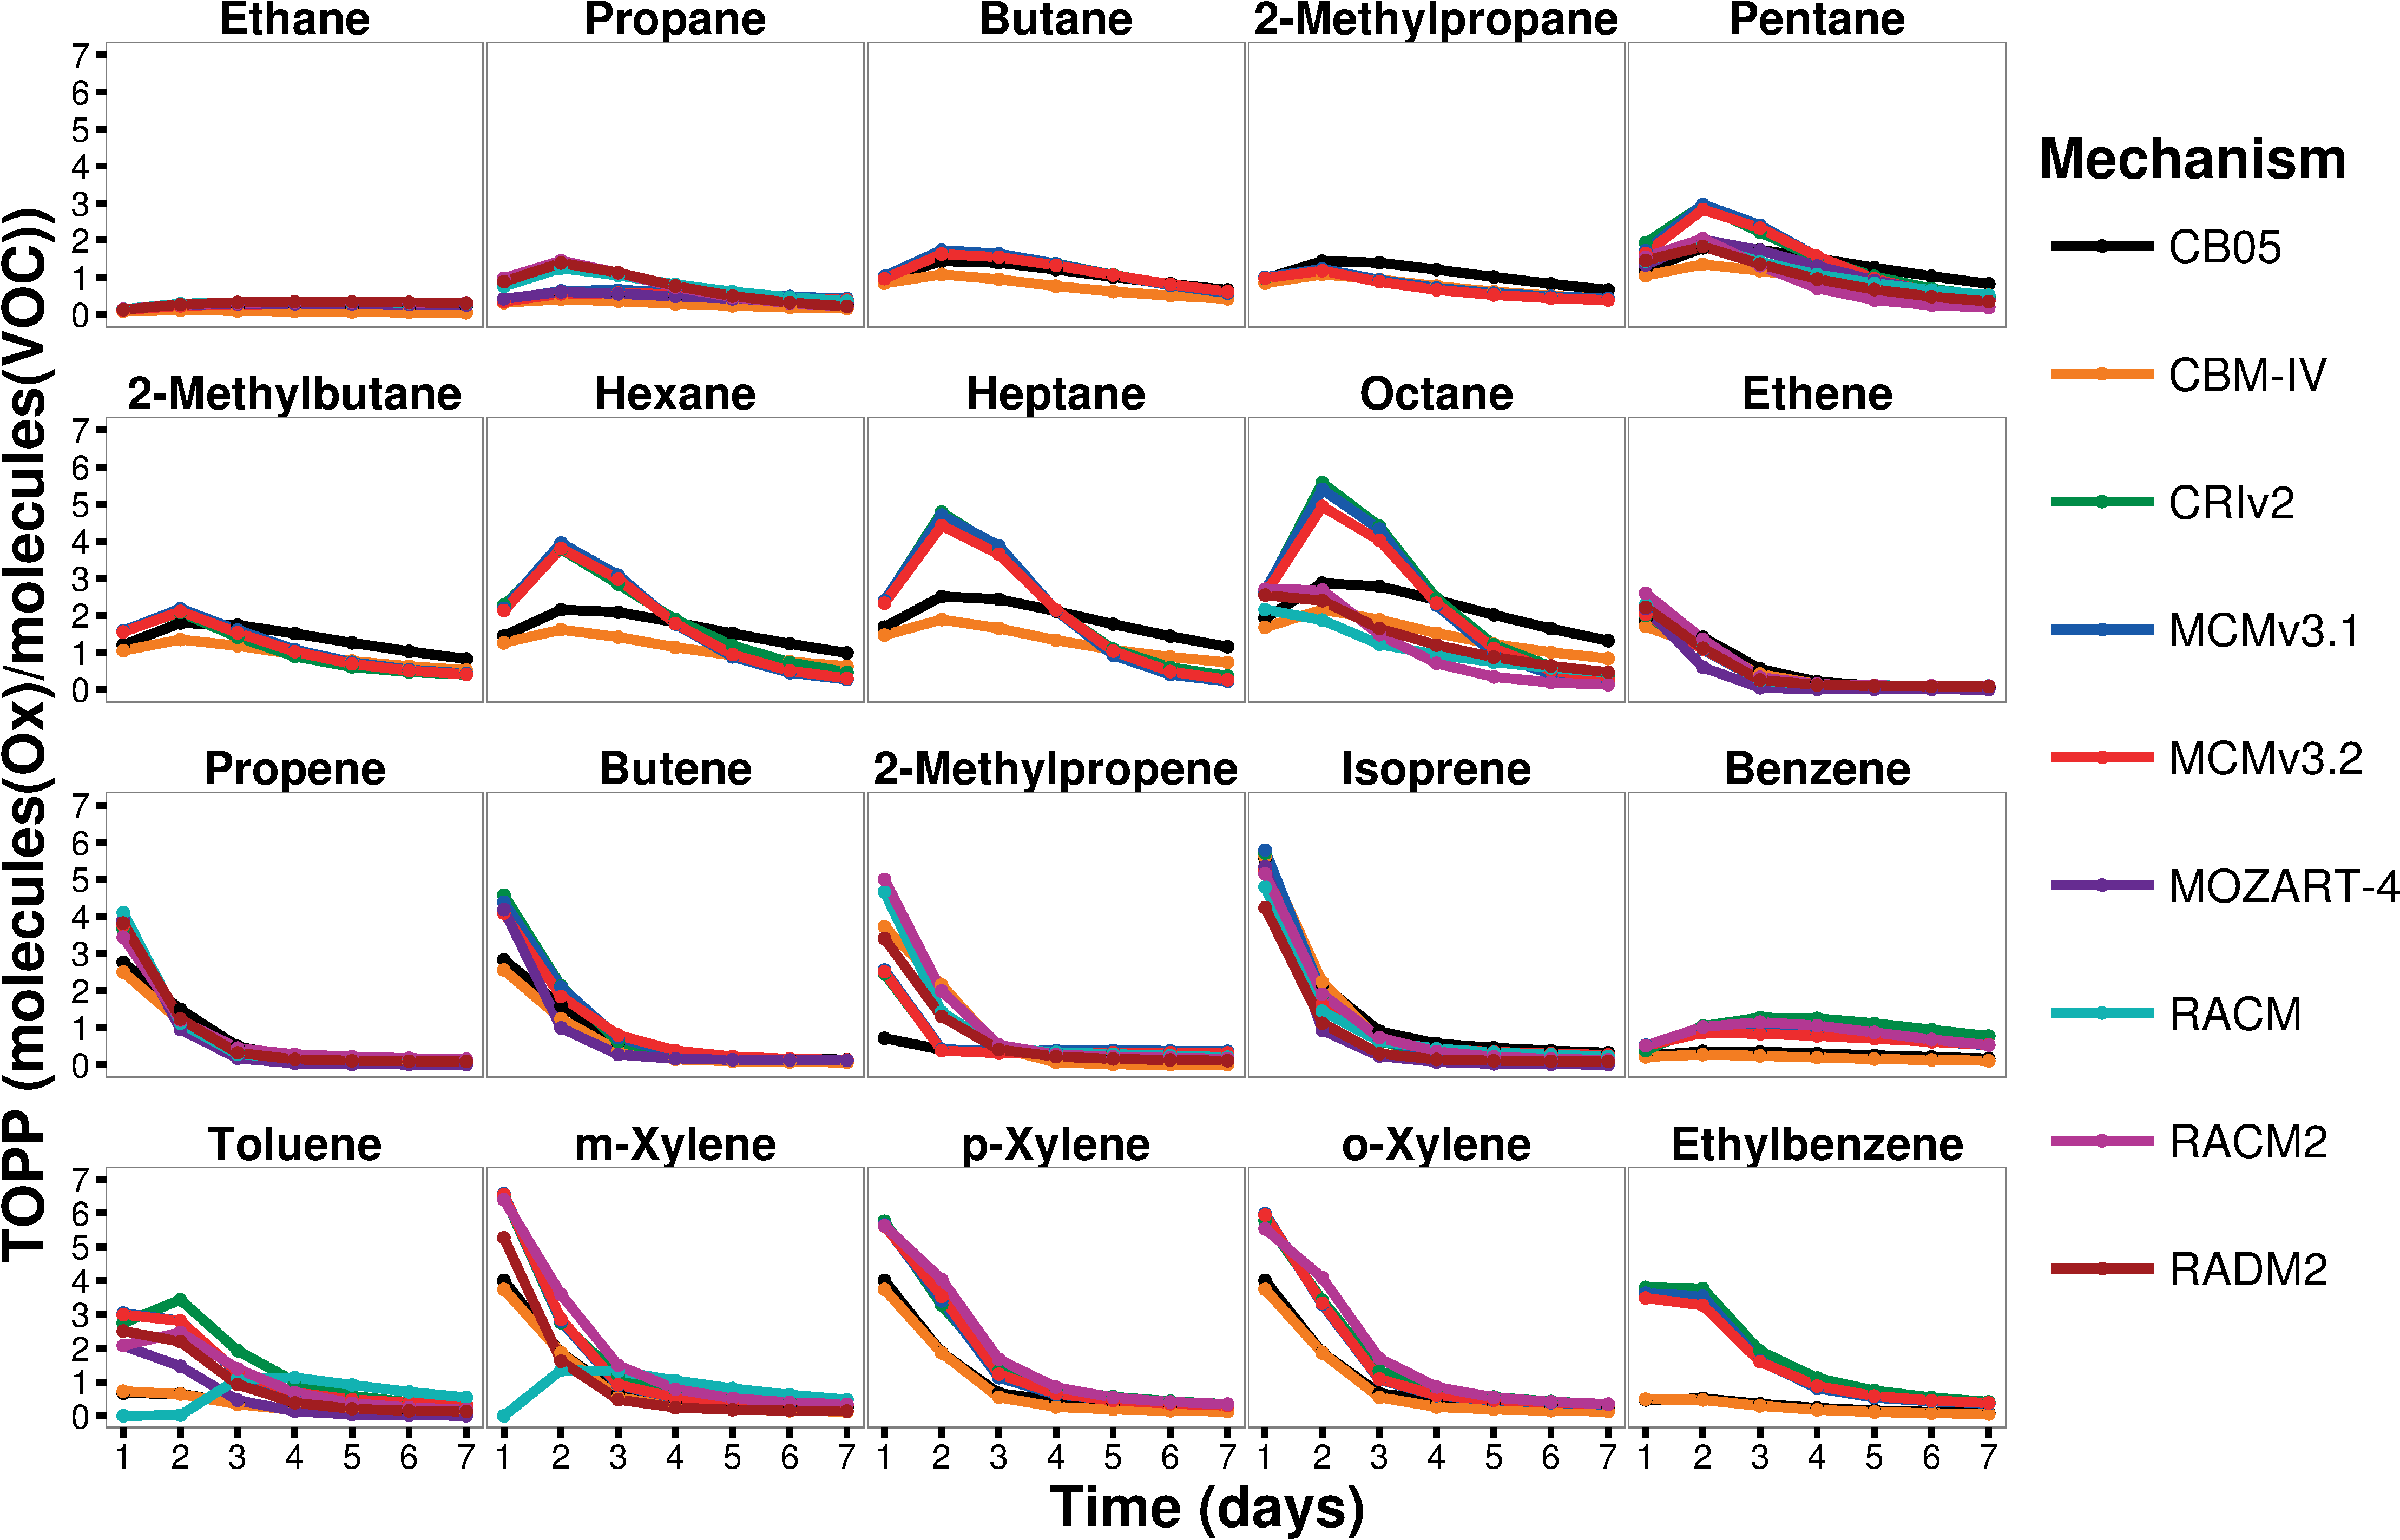
\includegraphics[width=\textwidth]{img/TOPP_daily_values_all_species}
    \vspace{0mm}
    \caption{TOPP value time series for all NMVOCs obtained with each mechanism.}
    \vspace{-4mm}
    \label{f:TOPP_dailies}
\end{figure}

The daily TOPP value time series of the NMVOCs are presented in \mbox{Figure \ref{f:TOPP_dailies}}. 
NMVOCs, such as ethene, whose degradation is described using dedicated mechanism species show similar time-dependent \ce{O_x} production.
Higher variability emerges between the time series of those NMVOCs represented by lumped mechanism species, such as pentane.

A second day \ce{O_x} production maximum of all alkanes is present by all mechanisms except RADM2, RACM and RACM2 representations of octane. 
Also, the MCM mechanisms have pronounced maxima that increase with carbon number.

Section \ref{ss:carbon_loss} outlines the impact on \ce{O_x} production from loss of carbon during VOC degradation.
Less-explicit mechanisms that break down the emitted VOC quicker than near-explicit mechanisms produce less \ce{O_x}.
In the case of octane, this break down proceeds so quickly that maximum \ce{O_x} production is on the first day. 
The supplement to this paper contains details of the octane analysis.

Aromatic VOC \ce{O_x} production has the most variability between mechanisms. 
In particular, zero \ce{O_x} production for toluene and m-xylene when using RACM.

\ce{O_x} production from toluene degradation in CBM-IV and CB05 is much lower than in the MCM v3.2.
This impacts \ce{O_x} production from ethylbenzene degradation as this is represented as \mbox{TOL + PAR}. 
Toluene degradation in RACM, CBM-IV and CB05 is summarised in Section \ref{sss:aromatic}.  

\subsubsection{Toluene Degradation in RACM, CBM-IV and CB05} \label{sss:aromatic}

\begin{figure}
    \centering
    \includegraphics[width=\textwidth]{img/TOL_Ox_intermediates}
    \vspace{0mm}
    \caption{The day-time \ce{O_x} production and consumption budgets from toluene degradation in \mbox{(a) MCM v3.2}, (b) RACM, (c) CBM-IV and (d) CB05.}
    \vspace{-4mm}
    \label{f:toluene_Ox}
\end{figure}

\ce{O_x} production and consumption day-time budgets due to toluene degradation in \mbox{MCM v3.2}, RACM, CBM-IV and CB05 are depicted in Figure \ref{f:toluene_Ox}. 
The tagging approach allows attribution of these budgets to the responsible organic reactions.

RACM chemistry results in net \ce{O_x} consumption on the first two days in contrast to the net \ce{O_x} production throughout the MCM v3.2 model run.
This is due to several \ce{O_x}-consuming reactions in RACM which are not present in the MCM.
The largest contribution is from the cresol OH-adduct mechanism species ADDC reaction with \ce{O3}. 
A fast rate constant \mbox{($5 \times 10^{-11}$ cm$^3$ s$^{-1}$)} was assigned to this reaction making it the main reaction pathway of ADDC. 
This reaction was included due to improved cresol product yields when comparing RACM predictions with experimental data \citep{Stockwell:1997}.

Other mechanisms that include cresol OH-adduct species do not include ozonolysis.
Including aromatic OH-adduct species ozonolysis in RACM results in non-representative \ce{O_x} production. 
This has been updated in RACM2 where aromatic OH-adduct species ozonolysis is no longer included.

\ce{O_x} production in CBM-IV and CB05 is mainly from the operator species XO2 which is a surrogate for organic peroxy radicals.
This is produced at various stages of toluene degradation and unlike typical organic peroxy radical degradation, the XO2 degradation chain ends after converting NO to \ce{NO2}.
Thus toluene degradation is unable to sustain \ce{O_x} production through further degradation products, as in other mechanisms.

\subsection{Radical Sources} \label{ss:radicals}

\begin{figure}
    \centering
    \includegraphics[width=\textwidth]{img/radical_production_analysis}
    \vspace{0mm}
    \caption{Net radical production day-time budgets for each mechanism. Net radical production calculated as the difference between radical and \ce{NO_x} yields. O1D represents the reaction of \ce{O(^1D)} with water vapour.}
    \vspace{-4mm}
    \label{f:radical_production} 
\end{figure} 

Maximum \ce{O_x} production was achieved by emitting the NO amount required to balance the radical source at each time step. 
Differences between mechanisms in radical production lead to different NO emissions.
Depending on the NO source, these differences may change the atmospheric regime represented by the mechanism.

Figure \ref{f:radical_production} illustrates the reactions responsible for day-time net radical production in each mechanism.
The reactions having net radical to \ce{NO_x} yield were determined for each mechanism, this was then multiplied by the reaction rate.

CBM-IV and CB05 have much higher net radical production rates on the first two days than any other mechanism.
Thus larger NO emissions are required for maximal \ce{O_x} production, indicating that CBM-IV and CB05 represent \ce{NO_x}-sensitive chemistry.

CBM-IV was developed for the high \ce{NO_x} conditions of urban and polluted regions \citep{Gery:1989}.
Hence, CBM-IV lacks low \ce{NO_x} chemistry such as organic peroxide formation.
CB05 includes oxygenated species so that organic peroxide chemistry is represented \citep{Yarwood:2005}.
However, CB05 net radical production rates are still significantly higher than other mechanisms.

The reaction of \ce{O(^1D)} with water vapour, \reactionref{r:O1D_H2O}, is the main radical source in each mechanism.%
\begin{reactionlist}%
    \reactionitem{\ce{O(^1D) + H2O}}{2 OH}{new}{r:O1D_H2O}
\end{reactionlist}%
\ce{O3} photolysis produces \ce{O(^1D)}, hence differences between the mechanisms in \ce{O3} amounts impacts \ce{O(^1D)} production.
Carbonyl photolysis is the main radical source from organic chemistry.
HCHO photolysis is the major carbonyl species impacting net radical production and this contribution is very similar between all mechanisms.

Methyl glyoxal photolysis impacts net radical production in each mechanism to varying degrees.
\mbox{Section \ref{sss:mglyox}} describes methyl glyoxal production of all mechanisms and explains these differences.

Most reduced mechanisms do not have sufficient carbonyl species to sustain radical production solely through photolysis.
VOC initial oxidation, \ce{RO2} reactions with NO and aromatic degradation product ozonolysis are used to sustain radical production in less-explicit mechanisms.
Examples of non-photolysis radical sources are given in Table \ref{t:thermal_radicals}.%

This analysis shows that different \ce{NO_x} conditions are required for maximum \ce{O_x} production between the mechanisms.
This may lead to different atmospheric regimes being represented in different mechanisms, resulting in different \ce{O_x} production levels.
These effects shall be further investigated in future work.
{%
    \renewcommand{\arraystretch}{1.3}
    \begin{table}
        \centering
        \small
        \begin{tabular}{lP{4.0cm}P{2.5cm}P{2.5cm}}
            \hline \hline
            \textbf{Mechanism} & \textbf{VOC OH Oxidation} & \textbf{\ce{RO2 + NO}} & \textbf{Ozonolysis} \\ \hline \hline
            RADM2 & HC5 + OH & NO + TCO3 & \\ \hline
            \multirow{2}{*}{RACM2} & & & DCB + O3 \\
            & & & EPX + O3 \\ \hline
            \multirow{3}{*}{CBM-IV} & C2H4 + OH & C2O3 + NO & \\
            & CH4 + OH & & \\
            & OH + PAR & & \\ \hline
            \multirow{3}{*}{CB05} & C2H6 + OH & CXO3 + NO & \\
            & C2H4 + OH & & \\
            & OH + PAR & & \\ \hline \hline
        \end{tabular}
        \vspace{1mm}
        \caption{Non-photolysis radical producing reactions.}
        \vspace{-4mm}
        \label{t:thermal_radicals}
    \end{table}
}%

\subsubsection{Methyl Glyoxal Production} \label{sss:mglyox}

\begin{figure}
    \centering
    \includegraphics[width=\textwidth]{img/MGLY_VOC_allocated_production_rates}
    \vspace{0mm}
    \caption{Methyl glyoxal production budgets allocated to parent VOCs in each mechanism.}
    \vspace{-4mm}
    \label{f:mglyox_budgets} 
\end{figure} 

Methyl glyoxal is represented in each mechanism -- MGLYOX in both MCM versions, CARB6 in CRI v2, CH3COCHO in MOZART-4 and MGLY in RADM2, RACM, RACM2, CBM-IV and CB05.
NMVOC degradation is the only source and Figure \ref{f:mglyox_budgets} shows the individual sources in each mechanism.

Isoprene and aromatic VOC degradation are the main methyl glyoxal sources in all mechanisms except RADM2, RACM and RACM2.
In these mechanisms, pentane and propane degradation produce the most methyl glyoxal.
MOZART-4 pentane degradation is also a source from the second day onwards.
The supplement shows the pentane degradation reactions influencing the methyl glyoxal production budget.

Acetone degradation in low-\ce{NO_x} conditions produces methyl glyoxal through the acetone peroxy radical reaction with other \ce{RO2} \citep{Fu:2008}.
Both MCM versions represent this chemistry however this route is not a major source as \ce{NO_x}-VOC-sensitive conditions are used.  
MOZART-4 also represents this chemistry with the rate constant four times faster than the MCM v3.2, leading to higher MOZART-4 production.

An additional methyl glyoxal production pathway from alkane degradation is included in RADM2, RACM and RACM2.
The NO + KETP reaction, KETP is the ketone peroxy radical, produces methyl glyoxal under high-\ce{NO_x} conditions.
This additional pathway leads to higher methyl glyoxal production from alkane degradation in these mechanisms.

Methyl glyoxal production from acetone degradation is not included in CRI v2, CBM-IV or CB05.
This chemistry is not included in CBM-IV and CB05 as high-\ce{NO_x} conditions are assumed.
In CRI v2, the acetone peroxy radical (RN8O2) skips methyl glyoxal production altogether and immediately produces \ce{CH3CO3}.
